\columnratio{0.55}
\begin{paracol}{2}
\switchcolumn[0]*%%%%%%%
\section{Provide / Inject}
\switchcolumn
\section{依赖注入}
\switchcolumn[0]*%%%%%%%
\begin{quote}
This page assumes you've already read the
\href{https://vuejs.org/guide/essentials/component-basics.html}{Components
Basics}. Read that first if you are new to components.
\end{quote}
\switchcolumn
\begin{quote}
此章节假设你已经看过了\href{https://cn.vuejs.org/guide/essentials/component-basics.html}{组件基础}。若你还不了解组件是什么,请先阅读该章节。
\end{quote}
\switchcolumn[0]*%%%%%%%
\subsection{Prop Drilling}
\switchcolumn
\subsection{Prop 逐级透传问题}
\switchcolumn[0]*%%%%%%%
Usually, when we need to pass data from the parent to a child component,
we use \href{https://vuejs.org/guide/components/props.html}{props}.
However, imagine the case where we have a large component tree, and a
deeply nested component needs something from a distant ancestor
component. With only props, we would have to pass the same prop across
the entire parent chain:
\switchcolumn
通常情况下,当我们需要从父组件向子组件传递数据时,会使用
\href{https://cn.vuejs.org/guide/components/props.html}{props}。想象一下这样的结构:有一些多层级嵌套的组件,形成了一颗巨大的组件树,而某个深层的子组件需要一个较远的祖先组件中的部分数据。在这种情况下,如果仅使用
props 则必须将其沿着组件链逐级传递下去,这会非常麻烦:
\end{paracol}

\begin{center} 
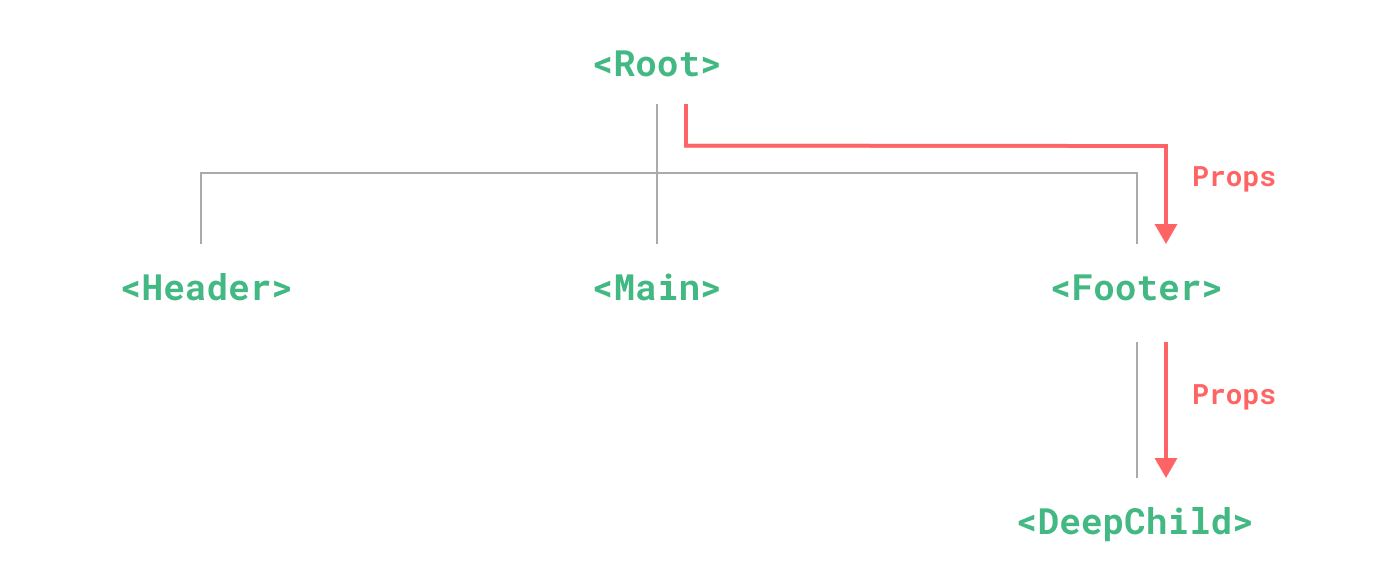
\includegraphics{./img/prop-drilling.11201220.png} 
\end{center}

\columnratio{0.55}
\begin{paracol}{2}
\switchcolumn[0]*%%%%%%%
Notice although the \texttt{\textless{}Footer\textgreater{}} component
may not care about these props at all, it still needs to declare and
pass them along just so \texttt{\textless{}DeepChild\textgreater{}} can
access them. If there is a longer parent chain, more components would be
affected along the way. This is called "props drilling" and definitely
isn't fun to deal with.
\switchcolumn
注意,虽然这里的 \texttt{\textless{}Footer\textgreater{}}
组件可能根本不关心这些 props,但为了使
\texttt{\textless{}DeepChild\textgreater{}}
能访问到它们,仍然需要定义并向下传递。如果组件链路非常长,可能会影响到更多这条路上的组件。这一问题被称为``prop
逐级透传'',显然是我们希望尽量避免的情况。
\switchcolumn[0]*%%%%%%%
We can solve props drilling with \texttt{provide} and \texttt{inject}. A
parent component can serve as a \textbf{dependency provider} for all its
descendants. Any component in the descendant tree, regardless of how
deep it is, can \textbf{inject} dependencies provided by components up
in its parent chain.
\switchcolumn
\texttt{provide} 和 \texttt{inject} 可以帮助我们解决这一问题。
\href{https://cn.vuejs.org/guide/components/provide-inject.html\#footnote-1}{{[}1{]}}
一个父组件相对于其所有的后代组件,会作为\textbf{依赖提供者}。任何后代的组件树,无论层级有多深,都可以\textbf{注入}由父组件提供给整条链路的依赖。
\end{paracol}

\begin{center} 
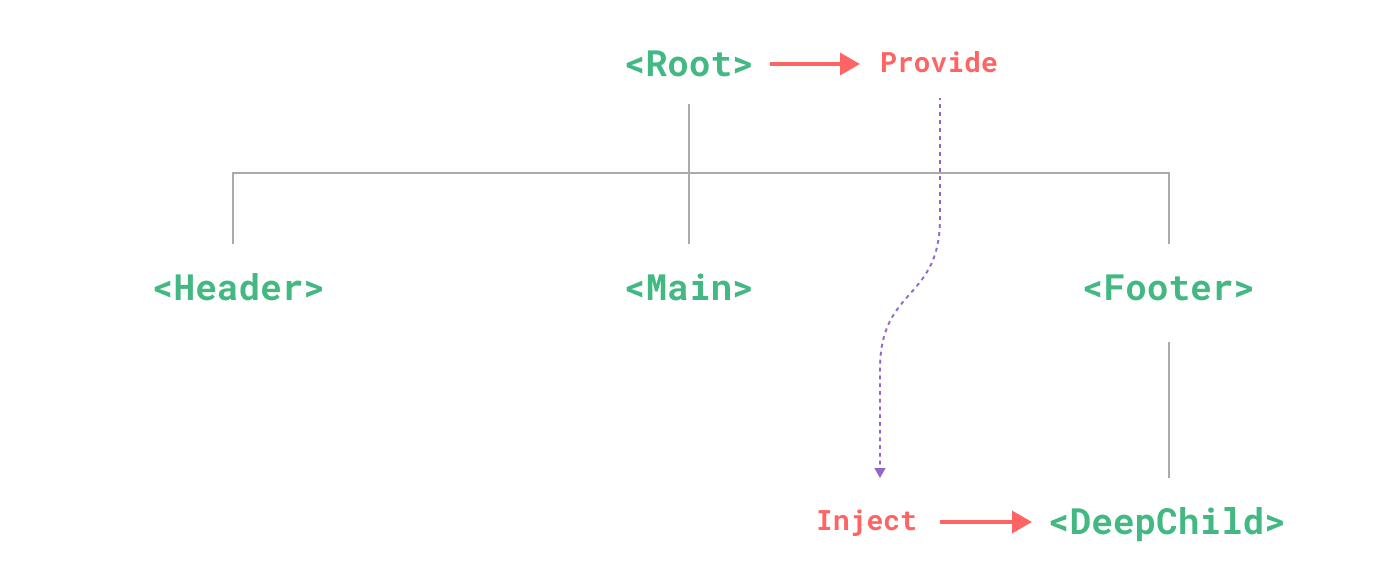
\includegraphics{./img/provide-inject.3e0505e4.png} 
\end{center}

\columnratio{0.55}
\begin{paracol}{2}
 
\switchcolumn[0]*%%%%%%%
\subsection{Provide}
\switchcolumn
\subsection{Provide (提供)}
\switchcolumn[0]*%%%%%%%
To provide data to a component's descendants, use the
\href{https://vuejs.org/api/composition-api-dependency-injection.html\#provide}{\texttt{provide()}}
function:
\switchcolumn
要为组件后代提供数据,需要使用到
\href{https://cn.vuejs.org/api/composition-api-dependency-injection.html\#provide}{\texttt{provide()}}
函数:
\switchcolumn[0]*%%%%%%%
\begin{codeHtml}
<script setup>
import { provide } from 'vue'
provide(/* 注入名 */ 'message', /* 值 */ 'hello!')
</script>
\end{codeHtml}
\switchcolumn
\begin{codeHtml}
<script setup>
import { provide } from 'vue'
provide(/* 注入名 */ 'message', /* 值 */ 'hello!')
</script>
\end{codeHtml}
\switchcolumn[0]*%%%%%%%
If not using \texttt{\textless{}script\ setup\textgreater{}}, make sure
\texttt{provide()} is called synchronously inside \texttt{setup()}:
\switchcolumn
如果不使用 \texttt{\textless{}script\ setup\textgreater{}},请确保
\texttt{provide()} 是在 \texttt{setup()} 同步调用的:
\switchcolumn[0]*%%%%%%%
\begin{codeJs}
import { provide } from 'vue'
export default {
  setup() {
    provide(/* 注入名 */ 'message', /* 值 */ 'hello!')
  }
}
\end{codeJs}
\switchcolumn
\begin{codeJs}
import { provide } from 'vue'
export default {
  setup() {
    provide(/* 注入名 */ 'message', /* 值 */ 'hello!')
  }
}
\end{codeJs}
\switchcolumn[0]*%%%%%%%
The \texttt{provide()} function accepts two arguments. The first
argument is called the \textbf{injection key}, which can be a string or
a \texttt{Symbol}. The injection key is used by descendant components to
lookup the desired value to inject. A single component can call
\texttt{provide()} multiple times with different injection keys to
provide different values.
\switchcolumn
\texttt{provide()}
函数接收两个参数。第一个参数被称为\textbf{注入名},可以是一个字符串或是一个
\texttt{Symbol}。后代组件会用注入名来查找期望注入的值。一个组件可以多次调用
\texttt{provide()},使用不同的注入名,注入不同的依赖值。
\switchcolumn[0]*%%%%%%%
The second argument is the provided value. The value can be of any type,
including reactive state such as refs:
\switchcolumn
第二个参数是提供的值,值可以是任意类型,包括响应式的状态,比如一个 ref:
\switchcolumn[0]*%%%%%%%
\begin{codeJs}
import { ref, provide } from 'vue'
const count = ref(0)
provide('key', count)
\end{codeJs}
\switchcolumn
\begin{codeJs}
import { ref, provide } from 'vue'
const count = ref(0)
provide('key', count)
\end{codeJs}
\switchcolumn[0]*%%%%%%%
Providing reactive values allows the descendant components using the
provided value to establish a reactive connection to the provider
component.
\switchcolumn
提供的响应式状态使后代组件可以由此和提供者建立响应式的联系。
\end{paracol}

\columnratio{0.55}
\begin{paracol}{2} 
\switchcolumn[0]*%%%%%%%
\subsection{App-level Provide}
\switchcolumn
\subsection{应用层 Provide}
\switchcolumn[0]*%%%%%%%
In addition to providing data in a component, we can also provide at the
app level:
\switchcolumn
除了在一个组件中提供依赖,我们还可以在整个应用层面提供依赖:
\switchcolumn[0]*%%%%%%%
\begin{codeJs}
import { createApp } from 'vue'
const app = createApp({})
app.provide(/* 注入名 */ 'message', /* 值 */ 'hello!')
\end{codeJs}
\switchcolumn
\begin{codeJs}
import { createApp } from 'vue'
const app = createApp({})
app.provide(/* 注入名 */ 'message', /* 值 */ 'hello!')
\end{codeJs}
\switchcolumn[0]*%%%%%%%
App-level provides are available to all components rendered in the app.
This is especially useful when writing
\href{https://vuejs.org/guide/reusability/plugins.html}{plugins}, as
plugins typically wouldn't be able to provide values using components.
\switchcolumn
在应用级别提供的数据在该应用内的所有组件中都可以注入。这在你编写\href{https://cn.vuejs.org/guide/reusability/plugins.html}{插件}时会特别有用,因为插件一般都不会使用组件形式来提供值。
\end{paracol}

\columnratio{0.55}
\begin{paracol}{2}
 
\switchcolumn[0]*%%%%%%%
\subsection{Inject}
\switchcolumn
\subsection{Inject (注入)}
\switchcolumn[0]*%%%%%%%
To inject data provided by an ancestor component, use the
\href{https://vuejs.org/api/composition-api-dependency-injection.html\#inject}{\texttt{inject()}}
function:
\switchcolumn
要注入上层组件提供的数据,需使用
\href{https://cn.vuejs.org/api/composition-api-dependency-injection.html\#inject}{\texttt{inject()}}
函数:
\switchcolumn[0]*%%%%%%%
\begin{codeHtml}
<script setup>
import { inject } from 'vue'
const message = inject('message')
</script>
\end{codeHtml}
\switchcolumn
\begin{codeHtml}
<script setup>
import { inject } from 'vue'
const message = inject('message')
</script>
\end{codeHtml}
\switchcolumn[0]*%%%%%%%
If the provided value is a ref, it will be injected as-is and will
\textbf{not} be automatically unwrapped. This allows the injector
component to retain the reactivity connection to the provider component.
\switchcolumn
如果提供的值是一个 ref,注入进来的会是该 ref
对象,而\textbf{不会}自动解包为其内部的值。这使得注入方组件能够通过 ref
对象保持了和供给方的响应性链接。
\switchcolumn[0]*%%%%%%%
\href{https://play.vuejs.org/\#eNqFUUFugzAQ/MrKF1IpxfeIVKp66Kk/8MWFDXYFtmUbpArx967BhURRU9/WOzO7MzuxV+fKcUB2YlWovXYRAsbBvQije2d9hAk8Xo7gvB11gzDDxdseCuIUG+ZN6a7JjZIvVRIlgDCcw+d3pmvTglz1okJ499I0C3qB1dJQT9YRooVaSdNiACWdQ5OICj2WwtTWhAg9hiBbhHNSOxQKu84WT8LkNQ9FBhTHXyg1K75aJHNUROxdJyNSBVBp44YI43NvG+zOgmWWYGt7dcipqPhGZEe2ef07wN3lltD+lWN6tNkV/37+rdKjK2rzhRTt7f3u41xhe37/xJZGAL2PLECXa9NKdD/a6QTTtGnP88LgiXJtYv4BaLHhvg==}{Full
provide + inject Example with Reactivity}
\switchcolumn
\href{https://play.vuejs.org/\#eNqFUUFugzAQ/MrKF1IpxfeIVKp66Kk/8MWFDXYFtmUbpArx967BhURRU9/WOzO7MzuxV+fKcUB2YlWovXYRAsbBvQije2d9hAk8Xo7gvB11gzDDxdseCuIUG+ZN6a7JjZIvVRIlgDCcw+d3pmvTglz1okJ499I0C3qB1dJQT9YRooVaSdNiACWdQ5OICj2WwtTWhAg9hiBbhHNSOxQKu84WT8LkNQ9FBhTHXyg1K75aJHNUROxdJyNSBVBp44YI43NvG+zOgmWWYGt7dcipqPhGZEe2ef07wN3lltD+lWN6tNkV/37+rdKjK2rzhRTt7f3u41xhe37/xJZGAL2PLECXa9NKdD/a6QTTtGnP88LgiXJtYv4BaLHhvg==}{带有响应性的
provide + inject 完整示例}
\switchcolumn[0]*%%%%%%%
Again, if not using \texttt{\textless{}script\ setup\textgreater{}},
\texttt{inject()} should only be called synchronously inside
\texttt{setup()}:
\switchcolumn
同样的,如果没有使用
\texttt{\textless{}script\ setup\textgreater{}},\texttt{inject()}
需要在 \texttt{setup()} 内同步调用:
\switchcolumn[0]*%%%%%%%
\begin{codeJs}
import { inject } from 'vue'
export default {
  setup() {
    const message = inject('message')
    return { message }
  }
}
\end{codeJs}
\switchcolumn
\begin{codeJs}
import { inject } from 'vue'
export default {
  setup() {
    const message = inject('message')
    return { message }
  }
}
\end{codeJs}
\end{paracol}

\columnratio{0.55}
\begin{paracol}{2}
\switchcolumn[0]*%%%%%%%
\subsubsection{Injection Default Values}
\switchcolumn
\subsubsection{注入默认值}
\switchcolumn[0]*%%%%%%%
By default, \texttt{inject} assumes that the injected key is provided
somewhere in the parent chain. In the case where the key is not
provided, there will be a runtime warning.
\switchcolumn
默认情况下,\texttt{inject}
假设传入的注入名会被某个祖先链上的组件提供。如果该注入名的确没有任何组件提供,则会抛出一个运行时警告。
\switchcolumn[0]*%%%%%%%
If we want to make an injected property work with optional providers, we
need to declare a default value, similar to props:
\switchcolumn
如果在注入一个值时不要求必须有提供者,那么我们应该声明一个默认值,和
props 类似:
\switchcolumn[0]*%%%%%%%
\begin{codeJs}
// 如果没有祖先组件提供 "message"
// `value` 会是 "这是默认值"
const value = inject('message', '这是默认值')
\end{codeJs}
\switchcolumn
\begin{codeJs}
// 如果没有祖先组件提供 "message"
// `value` 会是 "这是默认值"
const value = inject('message', '这是默认值')
\end{codeJs}
\switchcolumn[0]*%%%%%%%
In some cases, the default value may need to be created by calling a
function or instantiating a new class. To avoid unnecessary computation
or side effects in case the optional value is not used, we can use a
factory function for creating the default value:
\switchcolumn
在一些场景中,默认值可能需要通过调用一个函数或初始化一个类来取得。为了避免在用不到默认值的情况下进行不必要的计算或产生副作用,我们可以使用工厂函数来创建默认值:
\switchcolumn[0]*%%%%%%%
\begin{codeJs}
const value = inject('key', () => new ExpensiveClass(), true)
\end{codeJs}
\switchcolumn
\begin{codeJs}
const value = inject('key', () => new ExpensiveClass(), true)
\end{codeJs}
\switchcolumn[0]*%%%%%%%
The third parameter indicates the default value should be treated as a
factory function.
\switchcolumn
第三个参数表示默认值应该被当作一个工厂函数。
\end{paracol}

\columnratio{0.55}
\begin{paracol}{2}
 
\switchcolumn[0]*%%%%%%%
\subsection{Working with Reactivity}
\switchcolumn
\subsection{和响应式数据配合使用}
\switchcolumn[0]*%%%%%%%
When using reactive provide / inject values, \textbf{it is recommended
to keep any mutations to reactive state inside of the *provider*
whenever possible}. This ensures that the provided state and its
possible mutations are co-located in the same component, making it
easier to maintain in the future.
\switchcolumn
当提供 /
注入响应式的数据时,\textbf{建议尽可能将任何对响应式状态的变更都保持在供给方组件中}。这样可以确保所提供状态的声明和变更操作都内聚在同一个组件内,使其更容易维护。
\switchcolumn[0]*%%%%%%%
There may be times when we need to update the data from an injector
component. In such cases, we recommend providing a function that is
responsible for mutating the state:
\switchcolumn
有的时候,我们可能需要在注入方组件中更改数据。在这种情况下,我们推荐在供给方组件内声明并提供一个更改数据的方法函数:
\switchcolumn[0]*%%%%%%%
\begin{codeHtml}
<!-- 在供给方组件内 -->
<script setup>
import { provide, ref } from 'vue'
const location = ref('North Pole')
function updateLocation() {
  location.value = 'South Pole'
}
provide('location', {
  location,
  updateLocation
})
</script>
\end{codeHtml}
\switchcolumn
\begin{codeHtml}
<!-- 在供给方组件内 -->
<script setup>
import { provide, ref } from 'vue'
const location = ref('North Pole')
function updateLocation() {
  location.value = 'South Pole'
}
provide('location', {
  location,
  updateLocation
})
</script>
\end{codeHtml}
\switchcolumn[0]*%%%%%%%
\begin{codeHtml}
<!-- 在注入方组件 -->
<script setup>
import { inject } from 'vue'
const { location, updateLocation } = inject('location')
</script>
<template>
  <button @click="updateLocation">{{ location }}</button>
</template>
\end{codeHtml}
\switchcolumn
\begin{codeHtml}
<!-- 在注入方组件 -->
<script setup>
import { inject } from 'vue'
const { location, updateLocation } = inject('location')
</script>
<template>
  <button @click="updateLocation">{{ location }}</button>
</template>
\end{codeHtml}
\switchcolumn[0]*%%%%%%%
Finally, you can wrap the provided value with
\href{https://vuejs.org/api/reactivity-core.html\#readonly}{\texttt{readonly()}}
if you want to ensure that the data passed through \texttt{provide}
cannot be mutated by the injector component.
\switchcolumn
最后,如果你想确保提供的数据不能被注入方的组件更改,你可以使用
\href{https://cn.vuejs.org/api/reactivity-core.html\#readonly}{\texttt{readonly()}}
来包装提供的值。
\switchcolumn[0]*%%%%%%%
\begin{codeHtml}
<script setup>
import { ref, provide, readonly } from 'vue'
const count = ref(0)
provide('read-only-count', readonly(count))
</script>
\end{codeHtml}
\switchcolumn
\begin{codeHtml}
<script setup>
import { ref, provide, readonly } from 'vue'
const count = ref(0)
provide('read-only-count', readonly(count))
</script>
\end{codeHtml}
\end{paracol}

\columnratio{0.55}
\begin{paracol}{2}
 
\switchcolumn[0]*%%%%%%%
\subsection{Working with Symbol Keys}
\switchcolumn
\subsection{使用 Symbol 作注入名}
\switchcolumn[0]*%%%%%%%
So far, we have been using string injection keys in the examples. If you
are working in a large application with many dependency providers, or
you are authoring components that are going to be used by other
developers, it is best to use Symbol injection keys to avoid potential
collisions.
\switchcolumn
至此,我们已经了解了如何使用字符串作为注入名。但如果你正在构建大型的应用,包含非常多的依赖提供,或者你正在编写提供给其他开发者使用的组件库,建议最好使用
Symbol 来作为注入名以避免潜在的冲突。
\switchcolumn[0]*%%%%%%%
It's recommended to export the Symbols in a dedicated file:
\switchcolumn
我们通常推荐在一个单独的文件中导出这些注入名 Symbol:
\switchcolumn[0]*%%%%%%%
\begin{codeJs}
// keys.js
export const myInjectionKey = Symbol()
\end{codeJs}
\switchcolumn
\begin{codeJs}
// keys.js
export const myInjectionKey = Symbol()
\end{codeJs}
\switchcolumn[0]*%%%%%%%
\begin{codeHtml}
// 在供给方组件中
import { provide } from 'vue'
import { myInjectionKey } from './keys.js'
provide(myInjectionKey, { /*
  要提供的数据
*/ });
\end{codeHtml}
\switchcolumn
\begin{codeHtml}
// 在供给方组件中
import { provide } from 'vue'
import { myInjectionKey } from './keys.js'
provide(myInjectionKey, { /*
  要提供的数据
*/ });
\end{codeHtml}
\switchcolumn[0]*%%%%%%%
\begin{codeJs}
// 注入方组件
import { inject } from 'vue'
import { myInjectionKey } from './keys.js'
const injected = inject(myInjectionKey)
\end{codeJs}
\switchcolumn
\begin{codeJs}
// 注入方组件
import { inject } from 'vue'
import { myInjectionKey } from './keys.js'
const injected = inject(myInjectionKey)
\end{codeJs}
\switchcolumn[0]*%%%%%%%
See also:
\href{https://vuejs.org/guide/typescript/composition-api.html\#typing-provide-inject}{Typing
Provide / Inject}
\switchcolumn
TypeScript
用户请参考:\href{https://cn.vuejs.org/guide/typescript/composition-api.html\#typing-provide-inject}{为
Provide / Inject 标注类型}
\switchcolumn[0]*%%%%%%%
\href{https://github.com/vuejs/docs/edit/main/src/guide/components/provide-inject.md}{Edit
this page on GitHub}
\switchcolumn
\textbf{译者注}{[}1{]} 在本章及后续章节中,``\textbf{提供}''将成为对应
Provide 的一个专有概念
\end{paracol}